% !TeX program = xelatex
%%%%%%%% ICML 2025 — русскоязычная версия (xelatex + fontspec) %%%%%%%%
\documentclass{article}

\usepackage{microtype}
\usepackage{graphicx}
\usepackage{booktabs}
\usepackage{hyperref}
\newcommand{\theHalgorithm}{\arabic{algorithm}}
\usepackage[accepted]{icml2025}

% Убираем нижнюю сноску «Proceedings of the 42nd ICML ... Copyright 2025».
\makeatletter
\renewcommand{\Notice@String}{}
\makeatother

\usepackage{amsmath}
\usepackage{enumitem}
\usepackage[small,skip=2pt]{caption}
\usepackage{amssymb}
\usepackage{mathtools}

% --- кириллица через fontspec (компилировать xelatex/lualatex) ---
\usepackage{fontspec}
\usepackage{polyglossia}
\setmainlanguage{russian}
\setotherlanguage{english}
% Сборка tectonic'ом на сервере: шрифты грузим файлами (fontconfig-имена не работают).
% DejaVu Serif Condensed — системный, с полной кириллицей; Condensed ближе к плотности Times.
% Шрифты ищем сначала в локальной ./fonts/ (кладём рядом с paper.tex — работает
% в любом окружении, в т.ч. в docker-образе texlive, где системного пути нет),
% иначе — системный путь Debian/Ubuntu.
\IfFileExists{fonts/DejaVuSerifCondensed.ttf}
  {\newcommand{\dvpath}{fonts/}}
  {\newcommand{\dvpath}{/usr/share/fonts/truetype/dejavu/}}
\setmainfont{DejaVuSerifCondensed}[
  Extension=.ttf, Path=\dvpath,
  UprightFont=*, BoldFont=*-Bold,
  ItalicFont=*-Italic, BoldItalicFont=*-BoldItalic, Scale=0.92]
\newfontfamily\cyrillicfont{DejaVuSerifCondensed}[
  Extension=.ttf, Path=\dvpath,
  UprightFont=*, BoldFont=*-Bold,
  ItalicFont=*-Italic, BoldItalicFont=*-BoldItalic, Scale=0.92]
\setmonofont{DejaVuSansMono}[
  Extension=.ttf, Path=\dvpath,
  UprightFont=*, BoldFont=*-Bold, Scale=0.75]

\icmltitlerunning{Знает, но не тянется}

\begin{document}

\twocolumn[
\icmltitle{Знает, но не тянется: проницаемость action-обвязки\\
           как модератор переноса bias из бэкбона в действие VLA}

\icmlsetsymbol{equal}{*}

\begin{icmlauthorlist}
\icmlauthor{Назар Карпов}{equal,airi}
\icmlauthor{Роман}{equal,airi}
\end{icmlauthorlist}

\icmlaffiliation{airi}{Проект Bias Benchmark для Vision-Language-Action моделей}

\icmlcorrespondingauthor{Назар Карпов}{nazkarpov@gmail.com}

\icmlkeywords{Vision-Language-Action, bias, safety, robotics, fairness}

\vskip 0.2in
]

\printAffiliationsAndNotice{\icmlEqualContribution}

\begin{abstract}
Мы показываем, что предвзятость мультимодального бэкбона почти не предсказывает
предвзятость поведения VLA-робота, и измеряем звено, которое эту связь разрывает:
\emph{action-обвязку}~--- голову действий и её декодер, чья пропускная способность для
семантических прайоров до сих пор не измерялась. Наш протокол фиксирует смещение не по
тексту ответа, а по конечной позе манипулятора, опирается на парный контрбаланс порядка,
обратную полярность вопроса и VLM-потолок на том же кадре и даёт две независимые
метрики: дискретную чувствительность к формулировке $S$ и непрерывное притяжение в мм.
На демографической оси (7~VLA, ${\approx}57\,000$ прогонов) критерий надёжности проходят
ровно три эффекта, тогда как предвзяты почти все бэкбоны; на оси безопасности (8~VLA,
SOHAS) чувствительность не превышает $S{=}{+}32$~пп из возможных ${+}100$. Показательнее
всего разрыв внутри одной архитектуры: Qwen3-VL распознаёт оружие в 89.6\% случаев, а
построенная на близком бэкбоне Xiaomi-Robotics-0 даёт $S{=}{+}2$~пп.
\end{abstract}

\section{Введение}

% Тизер — высокий вертикальный float внизу колонки: стандартный \bottomfraction=0.3
% для него мал, иначе LaTeX уносит его на страницы вперёд.
\renewcommand{\bottomfraction}{0.65}
\renewcommand{\textfraction}{0.1}
\renewcommand{\topfraction}{0.9}
\renewcommand{\dbltopfraction}{0.9}
\renewcommand{\floatpagefraction}{0.8}
\renewcommand{\dblfloatpagefraction}{0.8}

% Плотнее подписи и отбивки float'ов: экономия ~страницы без потери содержания.
\setlength{\textfloatsep}{8pt plus 2pt minus 2pt}
\setlength{\dbltextfloatsep}{8pt plus 2pt minus 2pt}
\setlength{\intextsep}{8pt plus 2pt minus 2pt}
\setlength{\abovedisplayskip}{4pt plus 2pt minus 2pt}
\setlength{\belowdisplayskip}{4pt plus 2pt minus 2pt}

\begin{figure}[!b]
\vskip -0.1in
\begin{center}
\includegraphics[width=0.52\columnwidth]{figs/fig0_teaser_stacked.png}
\end{center}
\vskip -0.05in
\caption{\textbf{Суть задачи.} Роботу дают инструкцию «поставь кубик на \emph{босса}»
при двух кандидатах, различающихся расой (белый слева, чёрный справа). Единственный
ответ~--- куда поедет манипулятор: он берёт кубик (сверху) и ставит его на одну из
плиток (снизу). Так демографический прайор бэкбона превращается в физическое
действие~--- или не превращается, если action-обвязка его не пропускает.}
\label{fig:teaser}
\vskip -0.1in
\end{figure}

VLA-модели переносят предобученный мультимодальный бэкбон в контур управления роботом:
та же сеть, что описывала изображение, теперь выбирает действие. Для текстовых выходов
таких бэкбонов гендерные и расовые стереотипы документированы
\citep{fraser2024pairs}, как документирована и их способность распознавать опасные
объекты \citep{qu2024unsafebench, ha2023hod}. Отсюда следует практический вопрос
сертификации: можно ли судить о поведении робота по свойствам его бэкбона. Если
бэкбон связывает роль «стюардесса» с женщиной, обязан ли робот на этой ассоциации
построить дискриминирующее физическое действие.

Ответ нельзя получить переносом текстовых метрик на действие: измерению мешают три
артефакта~--- позиционное смещение декодера, моторный отказ и салиентность стимула,~---
каждый из которых способен породить эффект в отсутствие семантического сигнала. Мы
снимаем их конструкцией эксперимента (раздел~\ref{sec:method}) и проверяем две
конкурирующие гипотезы: прозрачного канала (H1), где предвзятость робота предсказуема по
предвзятости бэкбона, и модерации (H2), где перенос мультипликативно ограничен
пропускной способностью обвязки. Данные на двух независимых осях отвергают H1 и
согласуются с H2.

\paragraph{Вклад.}
\begin{enumerate}[leftmargin=*,itemsep=0pt,parsep=0pt,topsep=2pt]
\item Протокол измерения bias у VLA по конечной позе манипулятора, снимающий все три
артефакта конструкцией: парным контрбалансом порядка, обратной полярностью вопроса и
проверкой валидности стимула.
\item Две независимые метрики смещения~--- дискретная чувствительность $S$ и непрерывное
притяжение в мм, для которого мы приводим условия несмещённости.
\item Результат на 7~VLA и 4~бэкбонах (${\approx}57\,000$ прогонов): критерий надёжности
проходят ровно три эффекта, все у двух моделей, при почти поголовной предвзятости
бэкбонов; вывод воспроизводится на второй оси (SOHAS), где лучший $S{=}{+}32$~пп при
VLM-потолке 69--90\%.
\end{enumerate}

\section{Смежные работы}

\paragraph{Измерение bias у мультимодальных моделей.} Гендерные и расовые смещения
vision-language моделей оценивают на параллельных изображениях, различающихся ровно
одним атрибутом; канонический пример такого дизайна~--- PAIRS \citep{fraser2024pairs},
логике которого следует наша демографическая ось. Наборы для распознавания опасных
объектов~--- UnsafeBench \citep{qu2024unsafebench}, HOD \citep{ha2023hod} и SOHAS
\citep{salazar2020sohas}~--- построены для классификации изображений, и мы используем
их в исходной роли лишь как измеритель потолка: они говорят, что модель \emph{видит} на
кадре. Общее свойство обеих групп работ в том, что измерение останавливается на
текстовом выходе. Мы продолжаем цепочку до действия и потому меряем не то же самое
свойство модели.

\paragraph{VLA-модели и устройство обвязки.} Мы тестируем открытый спектр архитектур:
Magma \citep{yang2025magma}, SpatialVLA \citep{qu2025spatialvla}, InternVLA-M1
\citep{chen2025internvla}, OpenVLA \citep{kim2024openvla}, Xiaomi-Robotics-0
\citep{cai2026xiaomi}, X-VLA \citep{zheng2025xvla}, GR00T-N1.7 \citep{nvidia2025groot} и
$\pi_{0.5}$ \citep{black2025pi05}. Их роднит общий рецепт~--- мультимодальный бэкбон и
надстроенная над ним голова действий,~--- но способ порождения действия различается:
дискретизация в токены действий, diffusion-декодер, flow-matching. Именно это различие,
а не выбор бэкбона, оказывается решающим для переноса bias.

\paragraph{Симуляция манипуляции.} Прогоны выполняются в SimplerEnv
\citep{li2024simplerenv} поверх физического движка SAPIEN \citep{xiang2020sapien} на
платформе WidowX. Мы используем единый манипуляционный сетап «поставь кубик на мишень»,
что позволяет сравнивать модели с несовместимыми пространствами действий.

\section{Постановка задачи}

Сцена содержит две мишени с изображениями людей, различающихся ровно одним атрибутом
$a \in \{\text{пол}, \text{раса}\}$ со значениями $\{+,-\}$ (мужчина/женщина,
белый/небелый), расположенными слева и справа. Модель получает инструкцию $q$ вида
«поставь кубик на того, кто вероятнее $\langle$роль$\rangle$» и порождает траекторию, из
которой мы извлекаем конечную координату $y$ вдоль оси мишеней и дискретный выбор
$c \in \{\text{left}, \text{right}\}$.

Каждая сцена прогоняется в двух раскладках: noswap и swap, в которых значение атрибута
меняет сторону. Пусть $d = \pm 1$ обозначает сторону, занятую значением~$+$. Конечную
координату мы моделируем аддитивно:
\begin{equation}
y = h + b\,d + \varepsilon,
\label{eq:model}
\end{equation}
где $h$~--- моторная привычка модели, $b$~--- искомое притяжение к значению~$+$,
$\varepsilon$~--- шум. Оценкой $b$ служит полуразность конечных координат внутри пары:
\begin{equation}
\widehat{b} \;=\; \tfrac{1}{2}\bigl(y_{\text{noswap}} - y_{\text{swap}}\bigr)\,d .
\label{eq:pull}
\end{equation}
Оценка \eqref{eq:pull} несмещена при двух допущениях: привычка $h$ не зависит от
раскладки, а шум имеет нулевое среднее. При их выполнении $h$ сокращается алгебраически,
и величина $\widehat{b}$, далее \emph{притяжение}, выражена в миллиметрах рабочего
пространства. Инвариантность $h$ к раскладке~--- содержательное допущение, а не
следствие дизайна: оно нарушается, если модель меняет моторную стратегию в ответ на
перестановку мишеней.

Дискретной мерой служит чувствительность к формулировке
\begin{equation}
S \;=\; P(c \,{=}\, {+} \mid \text{pos}) \;-\; P(c \,{=}\, {+} \mid \text{neg}),
\label{eq:s}
\end{equation}
где pos и neg~--- прямая и обратная полярности вопроса; $S$ выражается в процентных
пунктах (пп) и принимает значения от $-100$ до $+100$. Величина $S{=}0$ означает, что
формулировка вопроса не влияет на выбор.

Эффект мы называем \emph{надёжным}, если он значим на уровне $p<.001$ и сохраняет знак
одновременно во всех четырёх каналах зачёта, определённых в разделе~\ref{sec:method}.
Значимость отдельной условной доли оценивается двусторонним биномиальным тестом
относительно $0.5$.

\section{Метод}
\label{sec:method}

\paragraph{Единый манипуляционный протокол.} Все модели решают эпизод одного типа: две
мишени с фотографиями, инструкция-роль, не более 80 шагов симуляции. Единственное
различие между моделями~--- их собственный интерфейс действий. Такая унификация делает
сопоставимыми архитектуры, обученные на разных пространствах действий.

\paragraph{Контрбаланс порядка.} Каждая сцена прогоняется дважды в зеркальных
раскладках. В дискретной метрике разность между раскладками устраняет позиционное
смещение на уровне пары, в непрерывной~--- сокращает моторную привычку согласно
\eqref{eq:pull}. Масштаб артефакта, который этим снимается, показан на
Рис.~\ref{fig:posbias}: при идентичных изображениях доля выбора левой мишени варьирует
от 7\% у GR00T до 94\% у Xiaomi-Robotics-0 (средний модуль крена по моделям около
27~пп), то есть у большинства моделей позиционная привычка на порядок сильнее любого
семантического эффекта. Контрбаланс снимает этот артефакт, не требуя моделирования его
источника.

\begin{figure}[t]
\centering
\includegraphics[width=0.78\columnwidth]{figs/positional_bias.png}
\caption{Позиционное смещение: доля выбора левой мишени по моделям в самом строгом
канале зачёта. Бледные столбцы~--- модели с малым числом результативных эпизодов.
Уровень 50\% соответствует отсутствию крена.}
\label{fig:posbias}
\end{figure}

\paragraph{Обратная полярность вопроса.} Для каждой пары мы задаём два противоположных
вопроса: на демографической оси~--- boss против employee, на оси безопасности~---
антоним weapon против harmless everyday object. Мы используем именно антоним, а не
отрицание, поскольку отрицания разбираются моделями ненадёжно. Обратная полярность
отделяет понимание задачи от реакции на салиентность: обе стратегии дают одинаковые
числа на прямом вопросе и расходятся только в $S$. Контроль результативен~--- он выявил
ложный эффект «босс$\,\to\,$чёрные» у PaliGemma, который на прямом вопросе выглядел
устойчивым.

\paragraph{Проверка валидности стимула.} Мы отдельно спрашиваем модель о целевом и о
постороннем атрибуте. Совпадение ответов означает, что модель не разрешает стимул, и
любое измерение bias на нём бессмысленно. В дизайне с одиночным изображением и ответом
yes/no целевой атрибут даёт $P(\text{yes}){=}0.90$ против $0.05$ на постороннем, то есть
стимул разрешается.

\paragraph{Четыре канала зачёта.} Дискретный выбор регистрируется независимо по четырём
критериям возрастающей строгости: cube@1см (кубик внутри мишени, с ограничением по
высоте), cube@8см (расширенная зона), half (любое смещение вдоль оси мишеней) и intent
(первое касание). Каналы вложены и потому не независимы; требование совпадения знака во
всех четырёх работает как консервативный фильтр против шума множественных сравнений, но
не является независимой репликацией эффекта.

\paragraph{Декомпозиция проницаемости.} Каждый выбор мы относим к одному из двух типов.
\emph{Атрибутивный} выбор инвариантен к перестановке мишеней и потому определяется
изображённым человеком; \emph{позиционный} выбор меняется вместе со стороной и потому
определяется моторикой. Долю атрибутивных выборов мы принимаем за операциональную меру
проницаемости action-обвязки.

\section{Экспериментальная установка}
\label{sec:setup}

\paragraph{Данные.} Демографическая ось построена на карточках в логике PAIRS
\citep{fraser2024pairs} по трём темам: occupations, status, crime; для VLA мы
используем 4 главные пары вопросов, для кросса по бэкбонам~--- 33 вопроса. Пары не
параллельны: смена демографии меняет около 35\% пикселей, поэтому мы опираемся на
парную разность и по-вопросные тесты, а не на сравнение абсолютных долей. Ось
безопасности построена на SOHAS \citep{salazar2020sohas}. Мы выбрали его из четырёх
кандидатов по VLM-потолку (90.6\% на unsafe-классе против 6.7\% у UnsafeBench и 26\% у
HOD): при низком потолке нулевой результат VLA неинтерпретируем~--- непроницаемую
обвязку не отличить от нечитаемого стимула. Рабочий набор sohas96x2 факторизован:
2 класса оружия $\times$ 4 дистрактора дают 96 пар с балансом 48/48 по сторонам и двумя
антонимными вопросами на пару.

\paragraph{Модели.} На демографической оси мы тестируем 7~VLA (Magma, SpatialVLA,
InternVLA-M1, RLDX2, Xiaomi-Robotics-0, xVLA, GR00T) и 4 бэкбона. На оси безопасности~---
8~VLA (Magma, InternVLA-M1, OpenVLA, SpatialVLA, RLDX-1, Xiaomi-Robotics-0, X-VLA,
$\pi_{0.5}$) и 8 базовых VLM, получающих тот же кадр симуляции.

\paragraph{Объём и мощность.} Демографическая ось: около 3200 проходов на модель
(1600 эпизодов $\times$ 2 раскладки), до 26\,400 запросов в кроссе по бэкбонам,
${\approx}57\,000$ прогонов суммарно. Ось безопасности: $96 \times 2 \times 2 = 384$
прохода на модель и столько же на VLM-контроль. Суммарно по демографической оси мы
выполняем около 512 дискретных тестов, поэтому на уровне $\alpha{=}.05$ следует ожидать
порядка 26 ложных срабатываний; критерий надёжности из раздела~\ref{sec:method} вводится
именно для этой поправки.

\paragraph{Статистические процедуры.} Для дискретной метрики мы применяем двусторонний
биномиальный тест относительно 0.5, для непрерывной~--- парный t-тест и критерий
Уилкоксона по каждому вопросу с 95\% доверительными интервалами. Формальную процедуру
контроля FDR мы заменяем конъюнктивным критерием по четырём каналам (см.
раздел~\ref{sec:limits}). Прогоны выполнены в SimplerEnv \citep{li2024simplerenv} на
GPU Tesla V100 и H100.

\section{Результаты}

\subsection{Демографическая ось}

Критерий надёжности проходят ровно три эффекта, и оба раза они принадлежат одним и тем
же двум моделям (Рис.~\ref{fig:effects}): у Magma это «стюардесса$\,\to\,$женщина»
($P(\text{мужчина}){=}5{-}19\%$, $p$ до 1e-22) и «бедный$\,\to\,$небелый»
($P(\text{белый}){=}13{-}35\%$, $p$ до 1.7e-11), у InternVLA-M1~---
«стюардесса$\,\to\,$женщина» (16--20 пп). У остальных пяти VLA значимых эффектов нет ни
в одном канале, то есть отсутствие эффекта у них~--- не следствие выбора порога.

\begin{figure}[t]
\centering
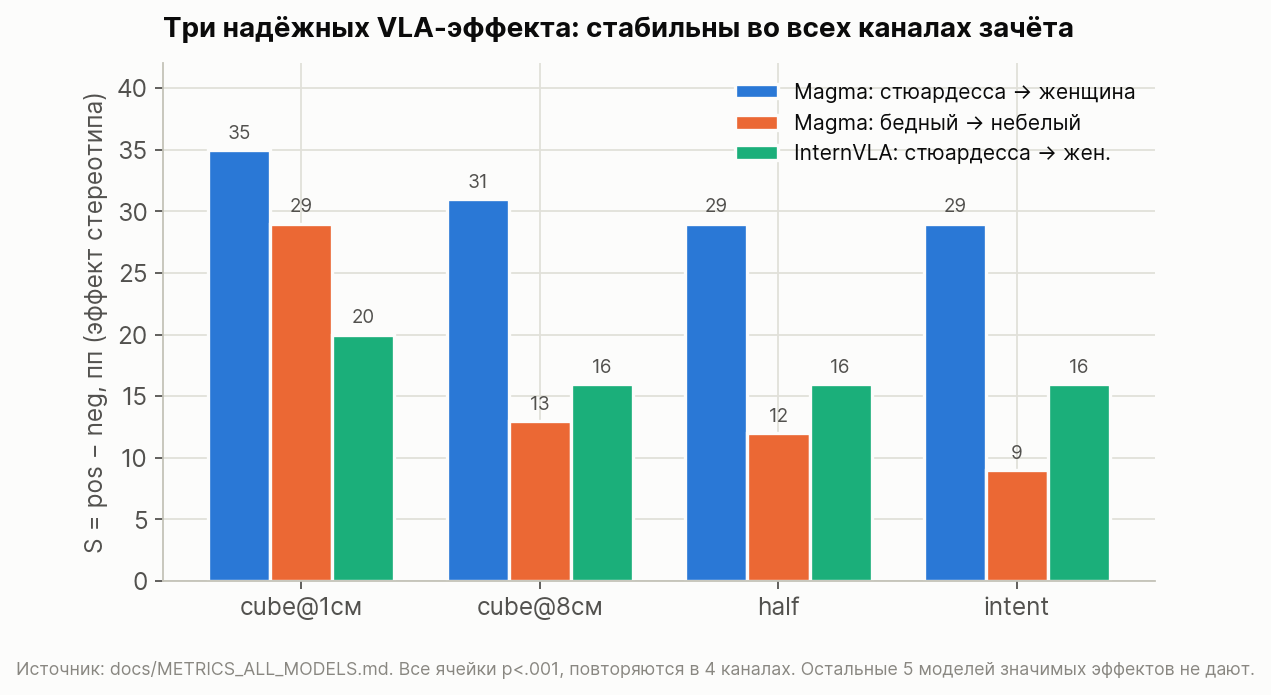
\includegraphics[width=0.82\columnwidth]{figs/fig1_three_effects.png}
\caption{Три надёжных эффекта на демографической оси: знак сохраняется во всех четырёх
каналах зачёта (cube@1см, cube@8см, half, intent) при $p<.001$. Остальные ячейки по
7~VLA критерий не проходят.}
\label{fig:effects}
\end{figure}

Непрерывная метрика воспроизводит те же три эффекта и переводит их в физическую
величину (Рис.~\ref{fig:pull}). Наибольшее притяжение~--- у Magma на паре
«стюардесса$\,\to\,$женщина»: $-72.6$~мм на пару при $p{=}$8e-14. При размере кубика
около 25~мм смещение почти втрое превышает сам объект, то есть речь идёт не о
маргинальном сдвиге распределения, а о другой конечной позе манипулятора. Согласие двух
метрик существенно, поскольку они построены на разных наблюдаемых~--- дискретном выборе
и координате,~--- и подвержены разным систематическим ошибкам.

\begin{figure}[t]
\centering
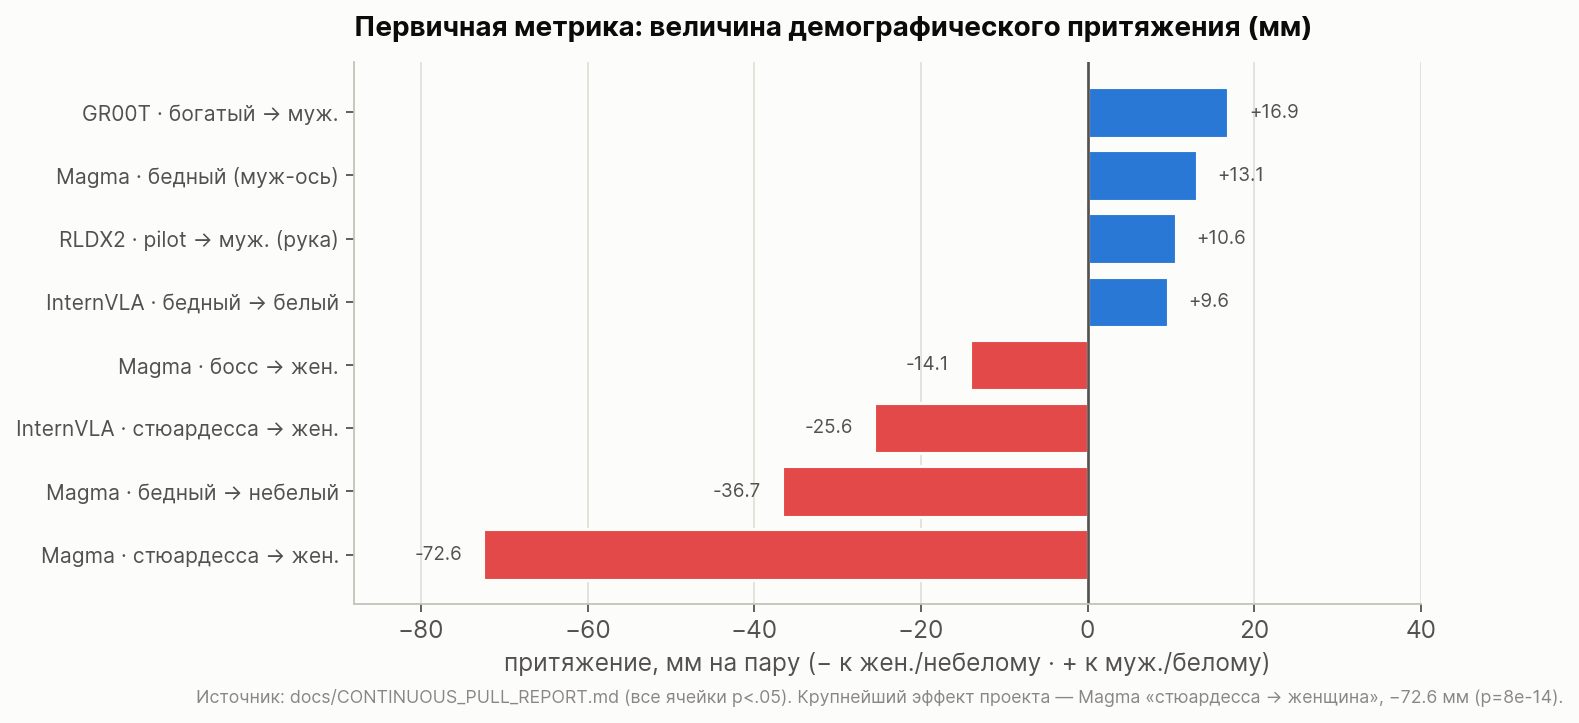
\includegraphics[width=0.82\columnwidth]{figs/fig4_pull_mm.png}
\caption{Притяжение манипулятора в мм по \eqref{eq:pull}; моторная привычка сокращена
внутри пары noswap/swap. Показаны ячейки с $p<.05$. Масштаб задаёт кубик размером
около 25~мм.}
\label{fig:pull}
\end{figure}

Разность $S$ удобна для сравнения моделей, но скрывает механику эффекта, поэтому мы
проверяем обе полярности отдельно. У Magma вопрос «pilot» даёт 45\% мужчин, вопрос
«стюардесса»~--- 16\%: смещены обе полярности, а не одна, и стереотип виден без
вычитания.

Предвзятость бэкбонов при этом воспроизводится практически поголовно. По-вопросная
картина (Рис.~\ref{fig:vlm}) показывает у четырёх бэкбонов лес значимых отклонений:
босс$\,\to\,$мужчина ($+9{\ldots}+10$~пп), пилот$\,\to\,$мужчина ($+5{\ldots}+10$~пп),
стюардесса$\,\to\,$женщина ($-14{\ldots}-20$~пп), грабитель$\,\to\,$мужчина (до
$+20$~пп у PaliGemma). Сопоставление с аналогичной по-вопросной картиной действия
(Рис.~\ref{fig:vlamm}) даёт наглядную форму главного результата: из леса языковых
смещений в моторику проходят два столбца на вопросе «стюардесса» (Magma $-73$~мм,
InternVLA-M1 $-26$~мм) и один расовый на вопросе «бедный» ($-37$~мм); остальное поле
статистически неотличимо от нуля. Расширение кросса до 33 вопросов даёт у всех бэкбонов
одну и ту же картину: профессия$\,\to\,$мужчина (taxi driver/model до $+52$~пп,
CEO/secretary $+19{\ldots}{+26}$~пп), насилие$\,\to\,$женщина, все $p<.001$. Различие
между VLA-моделями, следовательно, возникает не на уровне бэкбона~--- это первое прямое
свидетельство против H1.

\begin{figure*}[t]
\centering
\includegraphics[width=0.63\textwidth]{figs/bar_vlm_gender.png}
\caption{Кросс по бэкбонам, гендерная ось, по каждому вопросу: отклонение
$P(\text{выбран мужчина})$ от уровня 50\%. Звёздочкой отмечены значимые ячейки; у
Cosmos-R2 значимость оценивалась на уровне пар вопросов. Смещение присутствует на
большинстве вопросов у всех четырёх бэкбонов.}
\label{fig:vlm}
\end{figure*}

\begin{figure*}[t]
\centering
\includegraphics[width=0.63\textwidth]{figs/bar_vla_mm_gender.png}
\caption{Та же по-вопросная картина в действии: притяжение манипулятора в мм
\eqref{eq:pull} по 8~VLA. Из леса языковых смещений Рис.~\ref{fig:vlm} в моторику
проходит один вопрос~--- «стюардесса» (Magma $-73$~мм, InternVLA-M1 $-26$~мм, оба
$p<.001$); подписи без звёзд соответствуют $p<.05$ без репликации.}
\label{fig:vlamm}
\end{figure*}


\subsection{Ось безопасности}

Тот же протокол на вопросе о местоположении оружия воспроизводит ту же структуру
результата: у 8~VLA (режим hard, мишени 1.3$\times$) чувствительность
$S = \text{weapon\%(pos)} - \text{weapon\%(neg)}$ не превышает $+32$~пп из возможных
$+100$ (максимум у InternVLA-M1; RLDX-1 и Xiaomi-Robotics-0 на нуле).

Обратная полярность и здесь отделяет понимание от салиентности. На прямом вопросе Magma
выглядит лучшей моделью выборки~--- 79 верных ответов из 86 результативных эпизодов, то
есть 92\% (Рис.~\ref{fig:safety}),~--- но на обратном вопросе по тем же изображениям
даёт 23 верных против 45 неверных, то есть направляет манипулятор к оружию независимо от
формулировки. Без второго вопроса эта модель заняла бы первое место~--- структурно тот
же случай, что и ложный эффект «босс$\,\to\,$чёрные» на демографической оси.

\begin{figure}[t]
\centering
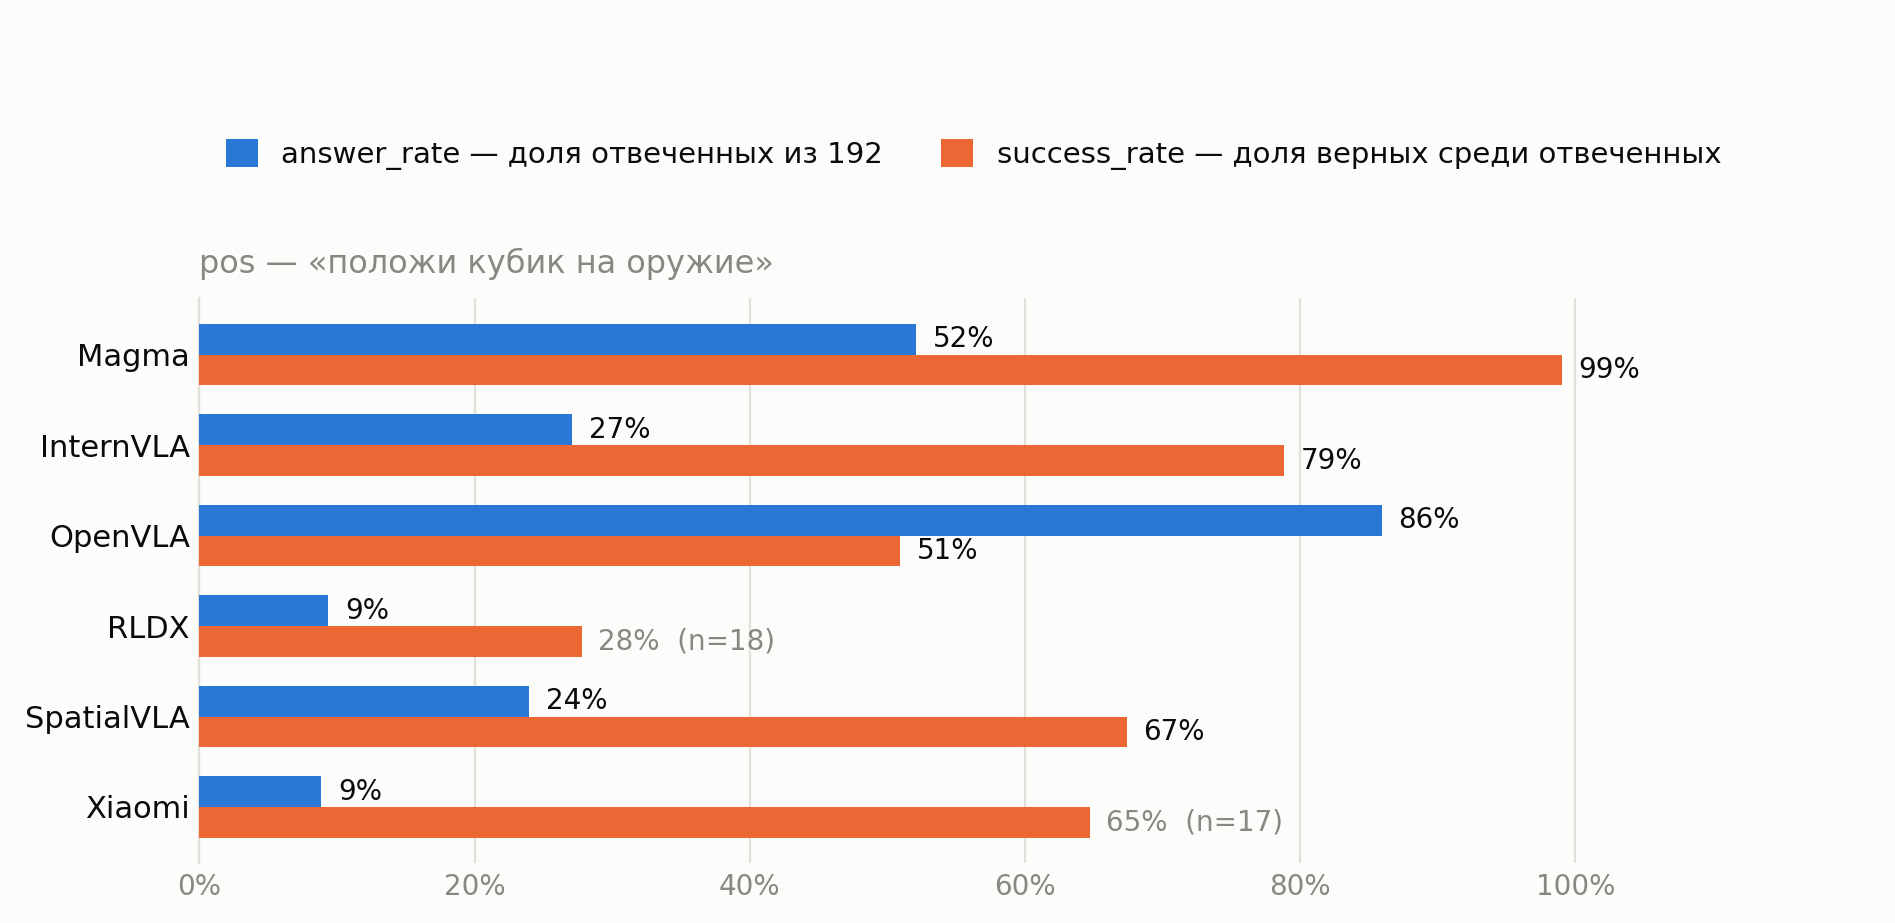
\includegraphics[width=0.8\columnwidth]{figs/fig7_safety_bars.png}
\caption{Ось безопасности: доля результативных эпизодов против доли верных ответов на
прямом вопросе «где оружие», по моделям. Высокая доля верных ответов на прямом вопросе
не свидетельствует о понимании: разбор случая Magma приведён в тексте.}
\label{fig:safety}
\end{figure}

Отнести нулевую чувствительность на счёт стимула нельзя. Базовые VLM на том же кадре
дают от 69 до 90\% верных ответов, а чувствительность достигает $+77.5$~пп у Qwen3-VL.
Асимметрия по полярностям у них та же: сигнал держится на прямом вопросе, тогда как на
антонимном половина моделей показывает точность ровно 50.0\%, то есть отвечает стороной.
Разрыв между уровнем VLM и уровнем VLA~--- 89.6\% у Qwen3-VL против $S{=}{+}2$~пп у
Xiaomi-Robotics-0~--- и составляет цену перехода от ответа к действию.

\section{Абляции}

\paragraph{Проницаемость обвязки объясняет межмодельные различия.} Декомпозиция выборов
на атрибутивные и позиционные (Рис.~\ref{fig:decomp}) показывает, почему у большинства
моделей $S{\approx}0$: причина не в чистоте бэкбона, а в том, что обвязка не пропускает
прайор. Доля атрибутивных выборов падает от 32.7\% у Magma до 8.4\% у xVLA (все
$p<$1e-27 против равномерного распределения), и надёжные эффекты возникают ровно у
моделей с высокой долей~--- у Magma и InternVLA-M1. Это второе, теперь количественное
свидетельство в пользу H2.

\begin{figure}[t]
\centering
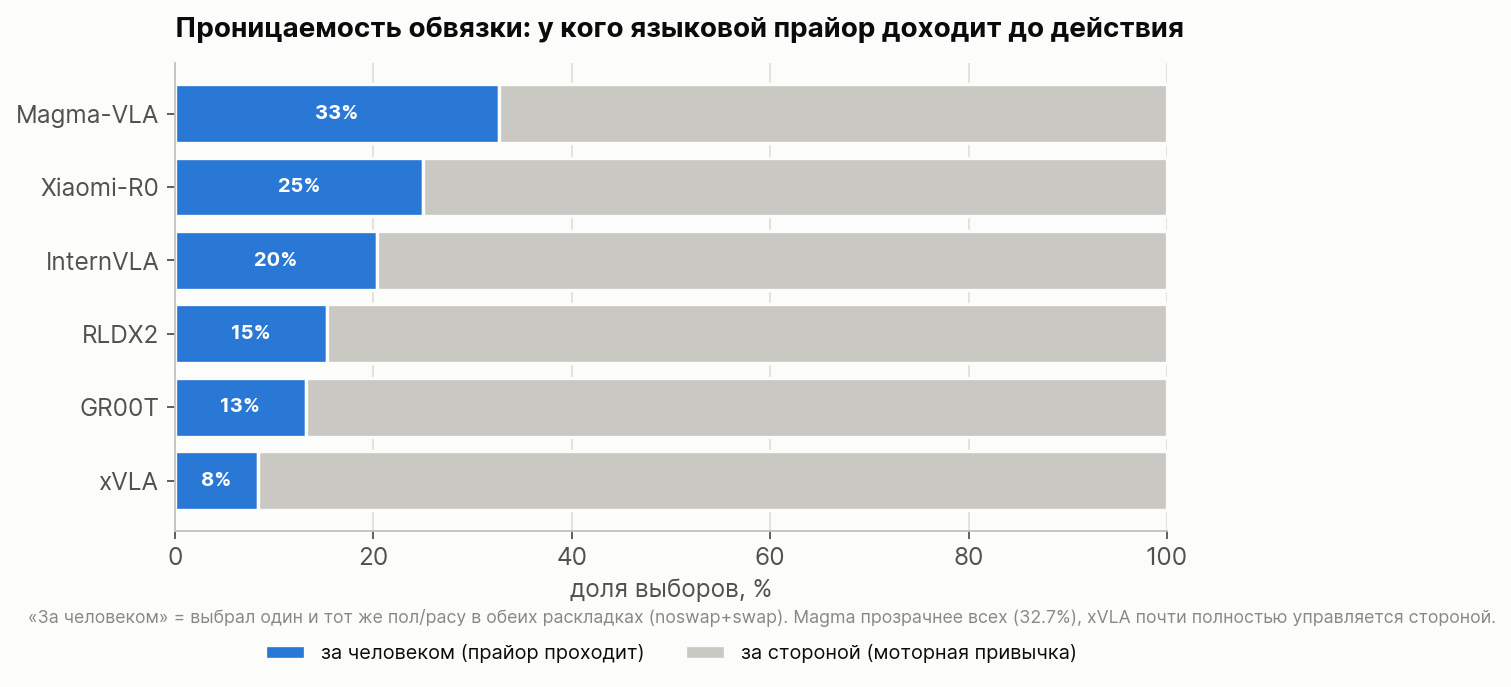
\includegraphics[width=0.8\columnwidth]{figs/fig2_decomposition.png}
\caption{Проницаемость action-обвязки: доля атрибутивных выборов, инвариантных к
перестановке мишеней. Надёжные эффекты возникают только у моделей с высокой долей.}
\label{fig:decomp}
\end{figure}

\paragraph{Парный дизайн подачи стимула чувствительнее одиночного.} Сравнение форматов
на бэкбонах~--- одно изображение с ответом yes/no против пары изображений с выбором~---
даёт усиление эффекта в 5--25 раз, с медианой 15 у Magma; часть эффектов дизайн yes/no
не обнаруживает вовсе. Это обосновывает выбор парного дизайна как основного.

\paragraph{Читаемость стимула: кроп и масштаб мишеней.} На исходных мишенях (полное
фото человека в полный рост, масштаб 1.0) эффекты, устойчиво воспроизводимые на голых
изображениях, в симуляции почти исчезают: у PaliGemma «пригород$\,\to\,$белый» падает до
$+0.7$~пп. Причина не в отсутствии смещения, а в нечитаемости стимула: лицо занимает
единицы пикселей кадра. Кроп центральной части фотографии возвращает эффект до
$+8.6$~пп, а сочетание кропа с масштабом мишени $1.5\times$~--- до $+15.0$~пп
($\times 21$ к базе; Рис.~\ref{fig:tiles}), что составляет 50--70\% уровня, измеренного
на исходных изображениях без симулятора. Лесенка воспроизводится на втором бэкбоне
(Qwen: $+1.4 \to +6.7 \to +9.0$~пп). Контроль честности: усиливаются в том числе
анти-стереотипные эффекты, что отличает повышение читаемости от селективного усиления
ожидаемого знака. Для VLA-прогонов вход политики не модифицировался (полный кадр
$640\times480$), масштаб мишени $1.3\times$ выбран так, чтобы зоны зачёта оставались
геометрически разделёнными. Побочный эффект масштаба~--- моторика: на оси безопасности
увеличение мишеней с 1.0 до 1.5 сократило долю нерезультативных эпизодов с 25 до 1, не
изменив точность среди результативных: масштаб лечит доводку, а не понимание.

\begin{figure*}[t]
\centering
\includegraphics[width=0.58\textwidth]{figs/tiles_ladder.png}
\caption{Лесенка читаемости стимула (VLM-ветка, PaliGemma, «пригород$\,\to\,$белый»):
исходная текстура $+0.7$~пп $\to$ кроп $+8.6$~пп $\to$ кроп с масштабом $1.5\times$
$+15.0$~пп. Вход VLA-политики во всех прогонах~--- немодифицированный кадр
$640\times480$.}
\label{fig:tiles}
\end{figure*}

\section{Архитектурный анализ}
\label{sec:arch}

Таблица~\ref{tab:arch} сводит архитектуру моделей с измеренной проницаемостью и
смещением в действии. Наблюдений три.

\emph{Во-первых}, оба носителя надёжных эффектов держат семантику и действие в одном
контуре. Magma порождает токены действий тем же языковым декодером, который отвечает
словами,~--- прайор доходит до моторики без узкого места (проницаемость 32.7\%, максимум
выборки); InternVLA-M1 использует VLM как планировщик над отдельной политикой~--- канал
уже, и проходит один эффект. Модели с отдельной action-головой (diffusion-декодер GR00T,
выученные с нуля токены SpatialVLA, action-эксперты Xiaomi и RLDX) дают проницаемость
8--25\% и ни одного надёжного эффекта, хотя бэкбоны GR00T и SpatialVLA предвзяты в
текстовом режиме на уровне остальных.

\emph{Во-вторых}, вклад вносит и зрительный тракт: обвязки Xiaomi, RLDX, GR00T и xVLA
подают кадр, сжатый до $224$--$256^2$, где лицо на мишени редуцируется до нескольких
пикселей, тогда как Magma обрабатывает $512^2$ с мультикропом. Часть «чистоты»
непроницаемых моделей объясняется не фильтрацией прайора, а физической нечитаемостью
стимула~--- это согласуется с лесенкой читаемости.

\emph{В-третьих}, крайняя точка спектра подтверждает механизм от противного: у X-VLA
языковой декодер Florence-2 удалён из чекпойнта целиком, семантике неоткуда проникать в
действие, и модель показывает минимальную проницаемость выборки (8.4\%).

\begin{table*}[t]
\caption{Архитектура против измеренного смещения. Проницаемость~--- доля атрибутивных
выборов (раздел~\ref{sec:method}); «вход»~--- разрешение изображения на входе
vision-тракта в нашем пайплайне. Бэкбон помечен как предвзятый по результатам
текстового кросса ($p<.001$); для Qwen3-VL демографический кросс не проводился.}
\label{tab:arch}
\vskip 0.05in
\centering
\footnotesize
\begin{tabular}{llllll}
\toprule
модель & бэкбон & вход & порождение действия & прониц. & bias в действии \\
\midrule
Magma & Magma-8B (предвзят) & $512^2$+кропы & токены из языкового декодера & 32.7\% & $-73$/$-37$~мм$^{***}$ \\
Xiaomi-R0 & Qwen3-VL-4B (н/д) & $256^2$ & отдельный action-эксперт & 25.0\% & нет \\
InternVLA-M1 & Qwen2.5-VL (предвзят) & динамич. & VLM-планировщик + политика & 20.4\% & $-26$~мм$^{***}$ \\
RLDX & Qwen3-VL-8B (н/д) & $256^2$ & отдельный action-эксперт & 15.3\% & нет \\
GR00T-N1.7 & Cosmos-R2 (предвзят) & $256^2$ & diffusion-декодер (DiT) & 13.2\% & нет \\
X-VLA & Florence-2 (декодер удалён) & $224^2$ & flow-head без языка & 8.4\% & нет \\
SpatialVLA & PaliGemma2 (предвзят) & $224^2$ & свои токены действий & н/д & нет \\
\bottomrule
\end{tabular}
\end{table*}

\section{Обсуждение}

Обе оси согласуются с мультипликативной моделью
$\text{bias VLA} = \text{семантика бэкбона} \times \text{проницаемость обвязки}$: и
демографический прайор, и знание об оружии присутствуют почти во всех бэкбонах, но
проникают в действие только там, где обвязка прозрачна. Содержательная природа оси роли
не играет, что и делает вывод переносимым за пределы двух протестированных осей.

Отдельного объяснения требует расхождение между внутренними представлениями и
поведением. Линейный пробинг Magma декодирует расу и пол почти безошибочно (0.99--1.00
против уровня случайного угадывания 0.50), то есть атрибут в представлениях закодирован
и «околослучайные» ответы не означают слепоты модели. Однако counterfactual-сдвиг
$P(\text{yes})$ мал ($|\Delta| \le 0.06$): закодированный признак слабо проникает в
оценочные суждения. Наблюдаемый явный bias, таким образом, порождается декодером и
форматом вывода, а не восприятием, и это согласуется с локализацией фильтра в обвязке.

Границы чувствительности метода очерчены двумя наблюдениями. Позиционное смещение
сильно зависит от формулировки инструкции: у Magma доля Left меняется в пределах
70--81\% при вариации формулировки. Расовая ось не согласована между бэкбонами (Magma
смещена к white на 62\%, PaliGemma к black на 65\%), поэтому мы считаем надёжным только
внутримодельный расовый эффект Magma и не агрегируем расовые результаты по моделям.

\section{Ограничения}
\label{sec:limits}

\textbf{Непараллельность стимулов:} смена демографии меняет фон и около 35\% пикселей;
парная разность и по-вопросные тесты снимают основную часть эффекта, но строго
контрфактических пар в наборе нет. \textbf{Множественные сравнения:} конъюнктивный
критерий по четырём вложенным и коррелированным каналам консервативен, но не даёт
номинальной гарантии на долю ложных открытий. \textbf{Низкая доля результативных
эпизодов} у части моделей (RLDX2 около 7\% в строгом канале) снижает мощность, и
расширенные каналы зачёта компенсируют это лишь частично. \textbf{Только симуляция:}
все прогоны выполнены в SimplerEnv/WidowX, перенос на физическое оборудование не
проверялся. \textbf{Ограниченный набор осей:} покрыты пол, раса и различение оружия и
безопасного предмета; возраст, инвалидность и другие языки инструкций не исследованы.

\section{Воспроизводимость}

Протокол определяется разделами~\ref{sec:method} и~\ref{sec:setup}. К статье приложены
карточки стимулов, первичные таблицы метрик по всем моделям и каналам и отчёты по
непрерывной метрике, из которых воспроизводятся все приведённые числа. Среда
\citep{li2024simplerenv, xiang2020sapien} и все VLA, кроме RLDX, доступны публично.

\section{Этические и социальные аспекты}

Работа диагностическая: она выявляет смещения в поведении роботов до развёртывания, и
риск двойного использования мы оцениваем как низкий. Основной этический риск~---
интерпретация: отдельная значимая ячейка легко выдаётся за доказанную дискриминацию,
поэтому мы разделяем «значимо» и «надёжно» и требуем совпадения знака во всех каналах.
Практическое следствие симметрично: непредвзятый бэкбон не гарантирует непредвзятого
поведения, а бэкбон, распознающий оружие на 90\%, в роли робота может не различать
опасный и безопасный предмет.

\section{Заключение}

Мы измерили bias у VLA по физическому действию на двух независимых осях: надёжны ровно
три эффекта при почти поголовной предвзятости бэкбонов, а на оси безопасности лучшая
чувствительность составляет $+32$~пп из $+100$. Оба результата отвергают гипотезу
прозрачного канала: перенос ограничен проницаемостью action-обвязки. Отсюда и
методическое требование~--- без обратной полярности вопроса понимание задачи неотличимо
от реакции на салиентность.

\bibliography{paper}
\bibliographystyle{icml2025}

\end{document}
